\chapter{Investigation of the association between the GP82AV mutation in Ebola virus and fatality rates}
\epigraph{The great tragedy of Science -- the slaying of a beautiful hypothesis by an ugly fact.}{Thomas Huxley (1825-1895) in \textit{Presidential Address at the British Association, Biogenesis and abiogenesis (1870)}.}


In this chapter I lay out and expand on my contribution to~\cite{Diehl2016}.
I scrutinise the association between being infected with a particular variant of the virus and the risk of dying, greatly extending the original analyses.

\section{Introduction}

One of the main scientific challenges emerging from the 2013-2016 Ebola virus disease (EVD) epidemic was understanding which factors contributed to such a large-scale epidemic.
While many such factors are likely to have been of environmental and socio-economical nature~\citep{Dudas2017}, the role of biological adaptation by the virus remains unclear.
In particular, evolutionary questions pertaining to the adaptation of the virus to humans and/or accelerated evolution and their impact on the trajectory of the epidemic assumed a central -- and often contentious -- role in the scientific literature (see e.g.~\cite{Holmes2016} and Section 5 in~\cite{Bausch2017}).

Ebola virus (EBOV) has a single-stranded negative-sense non-segmented RNA genome of around 18.9 Kb that encodes for at least 8 proteins (genes), amongst which the glycoprotein (GP), nucleoprotein (NP) and polymerase (L) are the most variable and useful for molecular epidemiology.
The GP gene codes for the virus glycoprotein, which is expressed on the surface of the viral particle as a transmembrane receptor~\citep{Takada1997}.
It is thought to be involved with  for receptor binding and membrane fusion and thus to be crucial for interaction with the host.
This also means the GP gene is one of most studied genes in the Ebola virus (EBOV) genome~\citep{Li2016}.

The present chapter concerns the study of the impact of a particular mutation on EVD fatality, namely a non-synonymous C-to-T substitution at nucleotide $6,283$ mutation resulting in the wild-type alanine (A) being replaced by a valine (V) at the 82nd aminoacid position, which interacts with the cell fusion receptor (NPC1).
This mutation, henceforth referred to as \verb|GP82AV| emerged early in the epidemic in Guinea (see Figure 1 in~\cite{Diehl2016}) and quickly spread through other countries and became dominant whereas the wild type (A) persisted in a few regions.
In~\cite{Diehl2016}, we analysed a set of clinical data for which there was information on which GP82 genotype the virus isolated from a patient had and also the EVD outcome (died/survived).
In that study, a positive association between  \verb|GP82AV| and risk of death (odds ratio: $2.09$, 95\% confidence interval [$0.94$, $4.64$]).

\subsection{Adaptation to humans}

This naturally raised questions of whether the virus had adapted to humans and become more virulent and/or transmissible.
\cite{Li2016} argue that no human adaptation occurred during the 2013-2016 Ebola epidemic using phylogenetic methods to show very little variation in evolutionary rates compared to previous epidemics.
As the authors themselves note, the evolutionary rate has little value in informing about the likelihood of adaptation to the host (discussed in detail in~\cite{Holmes2016}).
The authors also estimate selection on the GP gene and find no difference between the West African sequences and samples previous epidemics.
Their study did not however include any detailed experimental assessment of mutations in the GP gene and their impact on infectivity\footnote{In particular, the speculation that ``no non-synonymous substitutions occurred
on the GP gene coding sequences of EBOV that were likely to affect protein structure or function in any way.'' (pg. 7) was later challenged by~\cite{Urbanowicz2016} and~\cite{Diehl2016}.}.

\cite{Urbanowicz2016} and~\cite{Diehl2016} -- independently -- provide detailed experimental evidence on the impact of several point mutations in the GP gene on \textit{in vitro} infectivity in primate and human cells.
Both studies employ pseudotyped HIV particles to study viral infectivity of mutants and wild type in several types of cells.
These studies showed that viruses containing the \verb|GP82AV| mutation conferred increased human cell entry, and~\cite{Diehl2016} found a twofold increase in infectivity.
\cite{Urbanowicz2016} also found decreased infectivity in bat cells, suggesting an evolutionary adaptive trade-off.
An important observation is that these studies show adaptation to human cells, not to humans\footnote{This insightful remark is not my own but was instead made by Vincent Racaniello in his blog (http://www.virology.ws/2016/11/03/increased-infectivity-of-ebola-virus-glycoprotein-from-west-africa/).}.
This is an important distinction, because it highlights the fact that even if \verb|GP82AV| confers higher infectivity and tropism for human cells, it might have very little or no impact on viremia and disease progression. 

\subsection{Considerations about effect size}

While the studies by~\cite{Urbanowicz2016} and~\cite{Diehl2016} provide evidence that \verb|GP82AV| increases infectivity in human cells, the question of whether the increased infectivity could lead to more severe disease remains open.
It is entirely possible that the association between \verb|GP82AV| and fatality does not reflect any underlying causation.
I expect the outcome, i.e., whether an individual dies of EVD, to be dependent on a swathe of host- and population-specific factors.
An individual's age, sex, immune and nutritional status are expected to have a large contribution to risk of death\footnote{Importantly, this information is unfortunately not available for the data analysed in this chapter.}.
In addition, whether an individual can get access to medical attention depends on the availability of health care facilities in the region.

It is therefore important to scrutinise these estimates in order to assess their robustness to noise and confounding factors.
In other words, the main purpose of this chapter is to present a comprehensive analysis of the data in~\cite{Diehl2016} along with an in-depth discussion of the effect size of  the \verb|GP82AV| mutation in increasing fatality.
The analyses presented in that study are expanded in several ways: (i) I include more covariates in a more sophisticated model; (ii) I assess the robustness of the effect size estimates for \verb|GP82AV| by exploring (a) different model formulations and (b) several prior distributions for the effect size.

I include a discussion about errors in sign (S) and magnitude (M) in the framework of~\cite{Gelman2014}, explore several sources of uncertainty through the principled construction of prior distributions and address heterogeneity between locations using multilevel models.
Finally, I employ comparative method techniques to estimate heritability of viral loads and disentangle phylogenetic and clinical effects by conditioning on the shared ancestry between the samples.

\section{Methods}

In this chapter I shall make use of both orthodox (frequentist) and Bayesian methods, which might cause some confusion.
While I compute both confidence and credibility (or credible) intervals for various quantities, it is important to note that these are fundamentally different objects, in both construction and goal.
While confidence intervals are built with frequency guarantees in mind (e.g. a properly constructed 95\% confidence interval will contain the true parameter in 95\% of replicate experiments, on average), credibility intervals are constructed to give a 95\% probability that the true parameter is contained in the interval, without reference to replicated experiments/data sets.

\subsection{Data}

From the 1610 full EBOV genomes available, $316$ had information on cycle threshold (\ct) values and $299$ sequences had information on patient outcome (died/survived)\footnote{Please note there are small differences between the data described here and that analysed by~\cite{Diehl2016}.}.
The cycle threshold is a measure of how many polymerase chain reaction (PCR) cycles are necessary to obtain amplification of a given target sequence, and thus is directly related to the relative abundance of said sequence in the sample and can be used as a proxy for viral load, or the amount of virus DNA in a sample.
Since the cycle threshold (\ct) is inversely and non-linearly related to the amount of virus DNA in the sample, which in turn is thought to be correlated with viral load, I propose to transform \ct~in order to get the viral load, \verb|viral_load|$= -\log \text{C}t$.
While this transform ensures the sign of the coefficient in a regression setting is easier to interpret, magnitude is an entirely separate problem.
Since the main goal in this chapter is to study the effect of \verb|GP82AV| I will not pursue this issue any further.
There were $233$ sequences with complete information on \ct~and outcome, of which $221$ also had information about location.
When focussing solely on sequences from Guinea, we are left with $202$ sequences.

In order to aid modelling location-specific heterogeneity in case fatality rates, I collected a number of location-level predictors.
Specifically, I collected data on how many health centres, clinics and pharmacies there were in each prefecture (level 2 administrative unit).
These data were obtained from the Humanitarian Data Exchange initiative (\url{https://data.humdata.org/}).
In addition, in an effort to account for demographic, economic and epidemiological predictors, I also included information on population size and density, mean gridded economic output and travel time to the nearest settlement with more than $50,000$ inhabitants.
To keep coefficients comparable and facilitate prior specification, I transform continuous predictors by subtracting the mean and dividing by two standard deviations~\citep{Gelman2008}.
This ensures that coefficients for continuous predictors are comparable to those for binary predictors.

\subsection{Binary regression}
\label{sec:binreg}
Since the dependent variable is binary, I shall employ generalised linear modelling with a binary outcome $\boldsymbol Y \in [0, 1]^N$.
The model can be written as 
\begin{align}
 \label{eq:binglm}
 g(Y_i) &= \boldsymbol X_i^\intercal \boldsymbol\beta + \alpha  + \epsilon_i,\\
 \epsilon_i &\sim \text{Normal}(0, \sigma^2).
\end{align} 
where $g(\cdot)$ is the \textit{link function} and $\alpha$ is an intercept term.
Popular choices of link function include the logistic function $g(p) = \log\left(p(1-p)^{-1} \right)$, the probit link $g(p) = \boldsymbol\Phi^{-1}(p)$ -- where  $\boldsymbol\Phi^{-1}(\cdot)$ is standard normal inverse CDF -- and the cloglog link $g(p) = \log(-\log(1-p))$.
Each of these has its weaknesses and strengths, ranging from interpretability of the parameters to tail behaviour~\citep{Czado2006}.
The most common choice by far is the logistic link, mainly because it is easy to interpret parameter estimates; the estimate $\hat{\beta_i}$ represents the marginal log-odds of the $i-$th predictor/covariate.
The \textbf{odds ratio} $\text{OR}_i = \exp(\hat{\beta_i})$ gives a direct estimate of risk associated with the $i-$th predictor that is of great value in many scientific fields, particularly Epidemiology~\citep{Schmidt2008}.

The basic model in~(\ref{eq:binglm}) can be extended in several ways, including particular structures for the errors $\boldsymbol\epsilon$. 
In the following sections I detail multilevel\footnote{Also called ``random effects'' models. I prefer the term ``multilevel'' because it captures the true power of the framework: modelling data at several stages/level and pooling information across strata in a principled way. See sections 1.1 and 11.4 in~\cite{Hill2007} for a discussion on nomenclature.} extensions that are useful to the modelling task at hand.

\subsubsection{Multi-level models}
\label{sec:multilevel}

In several scientific applications, observations are made in batches or groups, e.g. students grouped within schools, disease cases grouped within locations, etc.
Multilevel models provide a framework for incorporating information at the individual level (e.g. the age and sex of a measured individual) with data at the group level (e.g. GDP per capita in a city)\citep{Hill2007}.
In the modelling situation tackled in this chapter, I am interested in including location-specific covariates that might be associated with risk of death from EVD.

For simplicity assume there is only one grouping factor and that observations come from $J$ groups.
Amongst more complicated structures, one can have (group-) varying intercepts, varying slopes or both.
For the purposes of this chapter, I will consider location-varying intercepts models, of the form
\begin{align}
 \label{eq:varyingintA}
  g(Y_{ij}) &= \boldsymbol X_{ij}^\intercal \boldsymbol\beta + \alpha_j  + \epsilon_{ij},\\
  \alpha_j &= \theta + \delta_j, \\
   \label{eq:varyingintB}
  \delta_j &= \boldsymbol Z_j^\intercal \boldsymbol\gamma.
\end{align}
where $\theta$ is an overall intercept, $\boldsymbol Z$ are group (location) level predictors, $\boldsymbol\gamma$ are the corresponding coefficients and the errors $\boldsymbol\epsilon$ are modelled as before (Eq.~\ref{eq:binglm}).
While this model is said to do \textit{partial pooling}, an alternative model where $\alpha_j\sim f(\cdot)$ assumes locations are i.i.d. and therefore does no pooling of information across locations.
A model where $\gamma_j = 0 \: \forall j$ (and therefore $\delta_j = 0 \: \forall j$) is said to be a \textit{complete pooling} model.

\textbf{Computational details}

I fit all generalised multilevel models using the probabilistic programming language Stan~\citep{Carpenter2017}, which allows the use  of Hamiltonian Monte Carlo (HMC,~\cite{Neal2011}) to approximate posterior distributions.
I run 4 independent chains of 5000 iterations with 2500 iterations discarded as warm-up.
I assessed convergence by visually inspecting parameter traces for stationarity and checking the $\hat{R}$ statistic~\citep{Brooks1998} was close to $1.0$..
To ensure appropriate mixing I also calculated effective sample sizes and checked they were above $200$.

\subsubsection{Prior modelling and effect size}
\label{sec:priors}

In this chapter I address the impact of prior specification for the regression model parameters in two ways: overall prior calibration, pertaining to the induced distribution of the outcome $\boldsymbol Y$ and the impact of several priors for the coefficient of the predictor of interest (absence/presence of \verb|GP82AV|) on the scientific conclusions one might draw from the model(s).

I propose to frame the assessment of effect sizes and prior construction in terms of \textbf{risk ratios} (RR), which are easier to understand and interpret.
Suppose we are comparing two groups, $g_0$ and $g_1$, for the occurrence of a given (binary) outcome.
An RR  of $1.03$ for instance means that individuals in $g_1$ have a $3\%$ higher chance -- \textit{i.e.} risk --  of developing the outcome compared to individuals in $g_0$\footnote{Hence $RR = p_1/p_0$, whereas $OR = p_1/(1-p_1) \div p_0/(1-p_0)$.}.
Since the models presented above (e.g.~\ref{eq:binglm}) are parametrised in terms of linear coefficients, we need to transform back and forth between RRs, ORs and coefficients:

\begin{align}
\label{eq:ORRRa}
 OR &= -\frac{(1-p_0)RR}{(p_0 RR -1)}, \\
 \label{eq:ORRRb}
 \beta &= \log(OR).
\end{align}

When modelling risk ratios for fatality, one needs to take into account the baseline \textbf{case-fatality rate} (CFR), $p_0$.
The maximum RR achievable for a given CFR is $RR_m = 1 + (1-p_0)/p_0$, and this can be used as an upper bound in the assessment of frequentist estimates and also the construction of priors.

\textbf{Informative priors}

I argue that we can use these functional forms to elicit informative priors for $\beta_{\text{GP82AV}}$ that encode specific hypotheses about the effect of \verb|GP82AV| on fatality rates.
The first step in constructing sensible priors is to understand the scale and variation of case-fatality rates.
I constructed a Beta distribution for $p_0$  with parameters $\alpha = 46.063$ and $\beta = 24.511$ using the information presented in page 6 of the meta-analysis by~\cite{Nyakarahuka2016}.
This information suggests the average CFR is $\mathbb{E}[p_0]= 0.65$, which in turn implies that $\mathbb{E}[R_m] = 1.54$,~\textit{i.e.} the average maximum risk ratio is about 54\%.
We can use this information to control the upper (right) tail of the distributions for $\beta_{\text{GP82AV}}$.
I propose we consider three scenarios
\begin{itemize}
 \item \textbf{Conservative:} there is very little chance there is an effect.
 RR should be $1$ with credibility interval (CI) $0.95, 1.05$;
 \item \textbf{Neutral:} we are agnostic about the effect; it could be protective or a risk factor.
 RR should be $1$ with 95\% CI $0.55, 1.45$;
 \item \textbf{Optimistic:} there is probably an effect of around $20$\% (RR = $1.20$), with a 95\% CI of $1.10, 1.45$;
\end{itemize}
To accommodate distributional idiosyncrasies such as different tail behaviour, I construct priors for each scenario using the log-normal and log-logistic families of distributions.
I present the results of this elicitation procedure in Figure~\ref{fig:informativePriors}.

\begin{figure}[!ht]
  \centering
  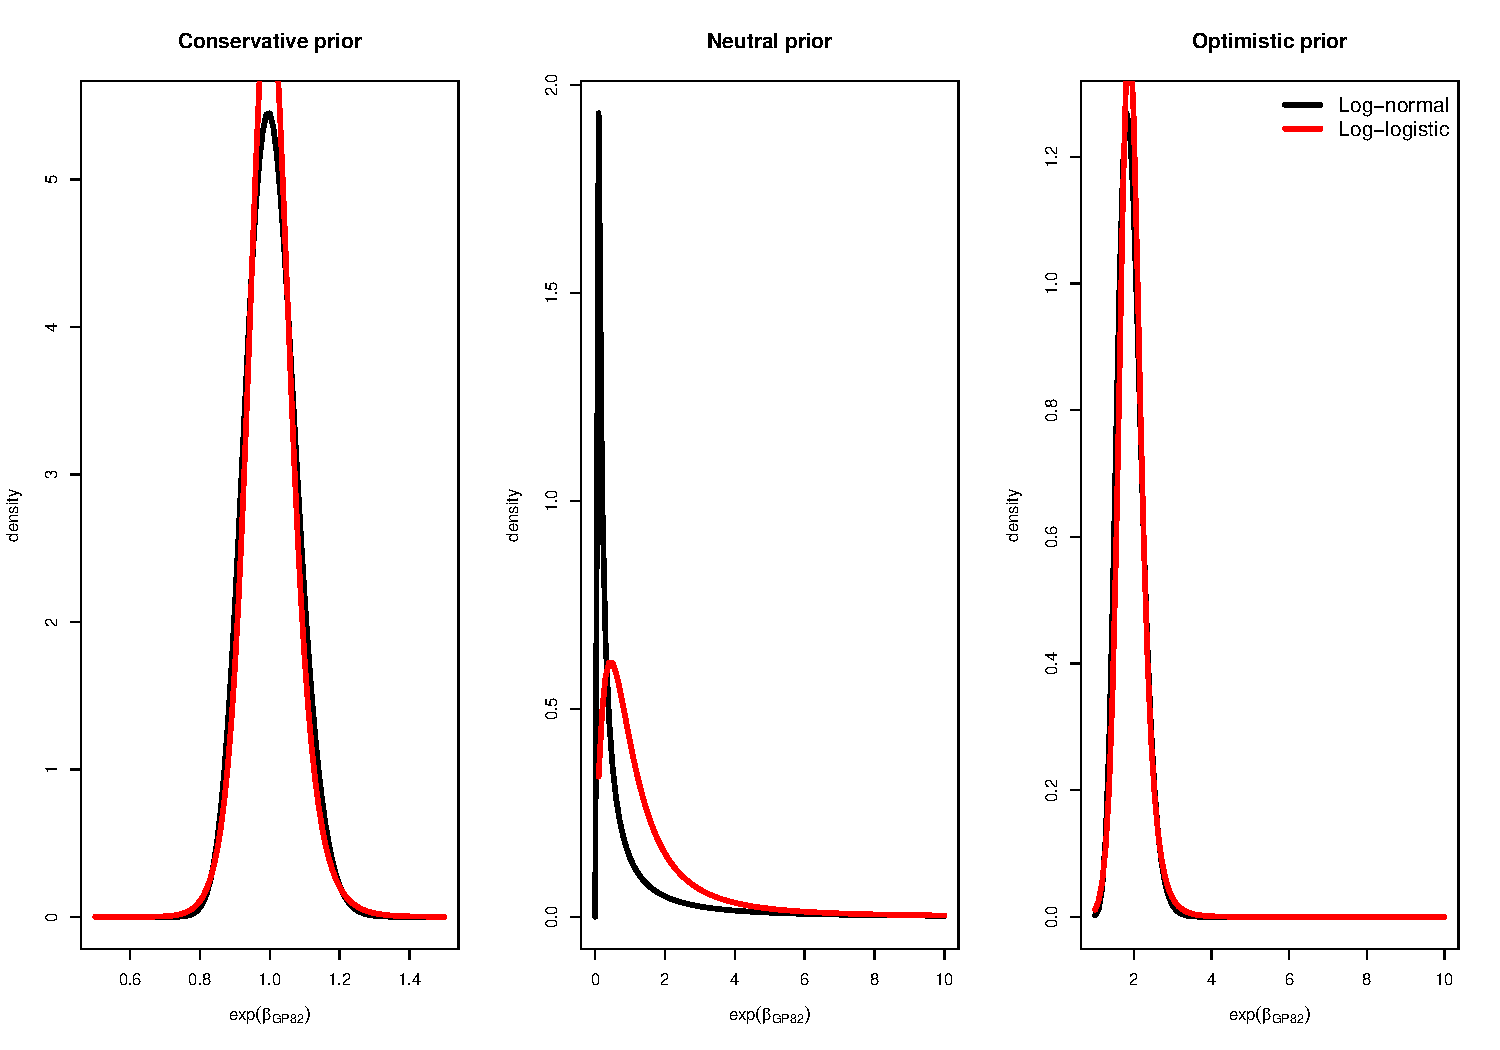
\includegraphics[scale=0.55]{\dir/figs/informative_prior_densities.pdf}
  \caption[Informative priors for the effect of GP82AV]{\textbf{Informative priors elicited for three scientific hypotheses about the effect of GP82AV.}
  I show conservative, neutral and optimistic priors constructed using a log-normal (black) and a log-logistic (red) distributions on the odds ratio ($\text{OR} = \exp(\beta_{GP82})$) for the GP82AV mutation.
  }
  \label{fig:informativePriors}
\end{figure}

\textbf{``Default'' and weakly-informative priors}

When performing inference with informative priors it is also good practice to explore sensitivity to prior specification by employing generic, weakly-informative default priors as a baseline.
In this chapter I look at several options for default priors commonly employed in the statistical literature.
Firstly, I explore an adaptation of the weakly-informative prior suggested by~\cite{Seaman2012}.
The authors study an example of logistic regression for coronary heart disease where the continuous predictor is age and they set $\sigma^2 = 25$.
Since the range of age is about $100-20 = 80$ years, I adapt my priors to have $\sigma^2 = r \times \frac{25}{80} = 1.63$, where $r = 2.59$ is the range of the \verb|viral_load| predictor (after standardisation).
I also consider the so-called g-prior~\citep{Zellner1986}, which scales the covariance matrix between coefficients proportional to the variance of the corresponding predictors $\boldsymbol X$, as $\pi(\boldsymbol\beta) \sim \text{Normal}_P(\boldsymbol 0, \frac{1}{g} \boldsymbol X^\prime\boldsymbol X)$.
Here I explore a g-prior with $g = N$ and a g-prior with an inverse-Gamma hyperprior on $g$ as discussed in~\cite{Liang2008}\footnote{It should be noted that the impact of the g-prior is minimised in our setting due to the scaling of the predictors. It is included here mostly for completeness.}.

A small caveat of eliciting the priors based on three quantities (mean, lower and upper 95\% quantiles) is that matching all three is sometimes not attainable.
Whenever this happened I chose to prioritise the mean and upper quantile for the neutral prior while focussing on the mean and lower quantile for the optimistic prior.
Elicitation  of the conservative prior encountered no such problems, mostly due to the small variances involved.

\textbf{Priors for the multi-level model parameters}

I assign a prior on $\theta$ such that $q = (1 + \exp(-\theta))^{-1}$ has a Beta distribution with parameters $\alpha = 46.063$ and $\beta = 24.511$.
For the no pooling model I assume $\alpha_j\sim \text{Cauchy}(0, 10)$, while for the partial pooling model I assign the location-level coefficients $\boldsymbol \gamma$ independent standard Gaussian priors.
For the overall intercept $\theta$, I opt for a Gaussian distribution with mean $0$ and standard deviation $5$.
The coefficients ($\boldsymbol\beta$ and $\boldsymbol\delta$) are given independent Cauchy priors with scale $5/2$ by default.

\subsection{Phylogenetic analyses}

Since viral genetic information is available for the clinical data discussed in this chapter, it is of interest to investigate the association between phylogeny -- of virus -- and the patient's outcome.

For the analyses outlined in this section, I estimated a time-calibrated phylogeny from the $299$ complete genomes using BEAST~\citep{Drummond2012}.
Data were divided into four partitions: coding regions with positions 1, 2 and 3 and intergenic region.
I used the HKY model~\citep{Hasegawa1985} model of nucleotide substitution along with Gamma-distributed rate heterogeneity and a log-normal relaxed clock that assumes among-branch variation in rates follows a log-normal distribution.

\subsubsection{Continuous trait analysis}
\label{sec:cta}

The first question I address is whether we can detect heritability in viral loads.
I study the association between phylogeny and viral load using a continuous diffusion model of trait evolution, as proposed by~\cite{Lemey2010}.
The idea is to model the trait under analysis as a process the evolves along a phylogeny following Brownian motion (BM), and perform inference by conditioning at the states (values) at the tips.
Additionally, I employ the Bayesian approach to Pagel's $\lambda$~\citep{Pagel1999} of~\cite{Vrancken2015} to estimate the heritability of viral load.
For the purposes of this chapter it is convenient to recall the interpretability of the phylogenetic correlation coefficient $\lambda_B$\footnote{The subscript denotes the fact that these estimates are Bayesian estimates derived from the posterior distribution of trees and hence accounting for phylogenetic uncertainty.}: if $\lambda_B = 0$ there is no correlation between phylogeny and the trait under analysis.
Conversely, $\lambda_B = 1$ corresponds to a setting where trait evolution reproduces a Brownian motion process along the phylogeny exactly.
Intermediate values represent the lack of adherence of the observed data to a BM.
These analyses used the same phylogenetic model described above, along with a boundary-avoiding Beta prior with parameters $\alpha = \beta = 2$ on $\lambda_B$.

\subsubsection{Phylogenetic regression}
\label{sec:phyloreg}

A key assumption of the models presented in Sections~\ref{sec:binreg}~and~\ref{sec:multilevel} is that the observations $\boldsymbol Y$ are independent.
Since EBOV relies on human to human transmission, that is, all cases are linked through a transmission chain\footnote{The hypothesis of multiple spillovers from the reservoir has been largely discredited~\citep{Baize2014, Gire2014}.}, this assumption is clearly violated.
One way to partially accommodate this fact is to assume that the phylogeny inferred from the sequences is a reasonable proxy for the dependence structure of the observations.
This idea underpins most of the comparative method and is the basis of the phylogenetic logistic regression (PLR) approach of~\cite{Ives2009}, which also accommodates binary covariates.
This is important because the main focus of this chapter is to study the effect of a binary variable, the absence/presence of the GP82AV mutation.

The idea behind PLR is to use the phylogenetic tree $\tau$ to construct a matrix $\boldsymbol W$ such that $W_{ii}$ is the distance from tip $i$ to the root and $W_{ij}$ is the length of the branch leading to the last common ancestor of $i$ and $j$.
This matrix is then used to formulate a phylogenetic variance-covariance matrix for $\boldsymbol Y$, $\boldsymbol V(\alpha)$:
\begin{align}
 \boldsymbol V(\alpha) &= \boldsymbol A^{1/2}  \boldsymbol C(\alpha)  \boldsymbol A^{1/2}, \\
  \boldsymbol C(\alpha) &= \exp\left(-2\alpha\left( \boldsymbol 1 - \boldsymbol W \right) \right), 
\end{align}
where $\boldsymbol 1$ is a $1 \times N$ unit vector, $\boldsymbol A$ is a diagonal matrix and $\alpha$ is a transition rate parameter controlling the evolution of the process along $\tau$ (see~\cite{Ives2009} for more details).
I use the \verb|phyloglm()| function in the~\textbf{phylolm} R package~\citep{Lam2014} to fit this model to the data using the phylogeny estimated as described above.
Confidence intervals were obtained with $500$ parametric bootstrap replicates.
 
\subsection{Type M and S errors}
\label{sec:MSerror}

In the framework of orthodox\footnote{Also called frequentist.} statistical inference and hypothesis testing, statements regarding reality are framed in terms of contrasts to a hypothesis.
The brief exposition of the Neyman-Pearson decision-theoretic paradigm here serves the purpose of motivating the analysis of type M and S errors and in no way reflects the richness of the research in orthodox statistics.
Please see e.g.~\cite{Casella2002} and references therein for a more detailed account.

More specifically, one is usually interested in studying the data $D$ under a \textit{null} hypothesis, $H_0$, which is chosen to encode the sceptical viewpoint.
Assuming $H_0$ holds true, one can use the hypothetical distribution of the data under $H_0$, $f(d; H_0)$\footnote{Notice I deliberately avoid the conditional probability notation, $f(d|H_0)$. For such a statement to be mathematically correct, one would have assign a valid probability measure over hypotheses, which would in turn lead us strictly outside the boundaries of orthodox Statistics.}, to answer questions such as ``how likely would we be to observe values of $D$ or more extreme assuming $H_0$ were true''?
Then, based on a pre-specified threshold for the probability $f(D; H_0)$, one can reject -- or fail to reject --  the null hypothesis $H_0$.

These testing procedures are usually calibrated in terms of error probabilities.
If one rejects $H_0$ when it is in fact true, we say a~\textbf{Type I error}  has been committed.
The \textit{false positive} rate $\alpha$ is the probability that a testing procedure will lead to a Type I error.
In contrast, when one fails to reject $H_0$ when it is false, one has committed a~\textbf{Type II error}.
The probability that a given testing procedure leads to a Type II error is denoted $\beta$.
It is useful to define the quantity $1-\beta$, the~\textbf{power} of the testing procedure.

\cite{Gelman2014} present an alternative perspective to the definition of errors in testing procedures.
They propose that we replace the notions of type I and II errors for the more intuitive concepts of errors about the~\textbf{magnitude (M)} and~\textbf{sign (S)} of the effect $t$.
The main idea is that if one is trying to estimate the effect $t$, there are two fundamental mistakes one could make: (i) obtain an estimate with the wrong sign or (ii) obtain an estimate that under- or over-estimates $t$.
Scientifically, a type S error could potentially lead to inferred causal links being reversed, while a type M error could lead to incorrect quantitative statements.

The key quantities in this framework are the measured effect size $\hat{t}$, the measured standard error (s.e.) $s$ and the~\textit{hypothesised} true effect size $t$.
From these, one can compute the distribution of the estimate $t_r$  that would be  obtained if the data collection and estimation procedure were to be replicated. 
With the distribution of the replicated estimates $t_r$ in hand, we are then prepared to compute three quantities~\citep{Gelman2014}:
\begin{itemize}
 \item The probability that $t_r$ exceeds the significance threshold, that is, the \textit{power};
 \item The probability that $t_r$ has a different sign from $t$,~\textit{i.e.} the type S error;
 \item The expected type M error, also called the exaggeration ratio, $a_e = E[|\frac{t_r}{t}|]$ which quantifies how far a replicated estimate would be from the true effect size if an statistically significant result were found. 
\end{itemize}

This framework lends itself well to the situation considered here, where we have an estimate of the effect of GP82AV on EVD fatality rates and would like to interrogate the study design and obtain estimates with respect to potential errors of both sign (is the mutation a protective or risk factor or none?) and magnitude (how much more/less risk of death from EVD stems from the absence/presence of GP82AV?).

An important caveat is that I do not know the true effect size $t$ and the literature is scant in terms of information that could be used to establish a reasonable value for $t$.
To address this I first use the bound derived in Section~\ref{fig:informativePriors} to restrict attention to effect sizes corresponding to risk ratios of less than $1.54$.
Here I postulate true effect sizes corresponding\footnote{Please recall that we need equations~\ref{eq:ORRRa}~and~\ref{eq:ORRRb} to convert between risk ratios and effect sizes.} to risk ratios of $1.05$, $1.10$, $1.20$ and $1.40$ and investigate the sensitivity of the calculations.
 
\section{Results and discussion}
\label{sec:results-discussion}

I begin by presenting the contingency table for GP82 genotype (A or V) and EVD outcome (died/survived) in Table~\ref{tab:rawData} and then providing raw estimates of the odds and risk ratios and associated standard errors.
A raw estimate for the odds ratio can be computed from the number of individuals infected with genotype GP82V that died (a) and survived (b) and likewise for cases of individuals infected with genotype GP82A that died (c) and survived (d).
The estimate for the raw odds ratio is then $m_{\text{OR}} = ad/bc$ and a $\alpha$\% confidence interval can be calculated as $\exp(m_{\text{OR}} \pm \phi^{-1}(\alpha/2) \cdot s_{\text{OR}})$, where $s_{\text{OR}} = \sqrt{(1/a) + (1/b) + (1/c) + (1/d)}$ is the standard error of the estimate.
Similarly, one can estimate the risk ratio as $m_{\text{RR}} = c(a + b)/a(c + d)$, with standard error $s_{\text{RR}} =  \sqrt{ (1/a + 1/c) - (1/(a + b) + 1/(c + d)) }$.

These calculations yield a raw odds ratio of $2.57$ $(1.34, 4.91)$ with standard error $0.33$ and a raw risk ratio of $1.23$ $(1.05, 1.45)$ with standard error $0.08$ for all of the available data, henceforth called complete data. 
When restricting attention to Guinea only, we obtain similar estimates of $2.78$ $(1.39, 5.54)$ with s.e. $0.35$  for the odds ratio and $1.26$ $(1.06, 1.49)$ with s.e. $0.09$ for the risk ratio. 

\begin{minipage}{\textwidth}  
\setcounter{mpfootnote}{\value{footnote}}
\renewcommand{\thempfootnote}{\arabic{mpfootnote}}
% \textsf{
\fontsize{9}{11}\selectfont
% \rowcolors{5}{gray!25}{white}
\begin{longtable}{ccc}
\caption[Contingency table for GP82AV and EVD fatality -- complete data.]{\textbf{Contingency table for GP82AV and EVD fatality -- complete data.} When restricting attention to Guinea, the numbers become $a = 106$, $b = 18$, $c = 53$ and $d = 25$.}
\label{tab:rawData}\\
 \hline
GP82 genotype/Outcome & Died & Survived\\ 
  \hline
V & $a = 130$ & $b = 23$ \\ 
A & $c = 55$ & $d = 25$ \\ 
   \hline
\end{longtable}
\setcounter{footnote}{\value{mpfootnote}}
% }
\end{minipage}

It would be desirable, however, to adjust these estimates for the effect of the continuous predictor, \verb|viral_load|.
This can be achieved by fitting a logistic generalised linear model with both \verb|viral_load| and \verb|GP82AV| as predictors (see Section~\ref{sec:binreg}), which yields estimates of $\beta_{\text{GP82AV}} =  0.75$ $(0.02,1.49)$ with standard error $0.37$, corresponding to an odds ratio of $2.13$ $(1.02, 4.44)$\footnote{Estimates for the data from Guinea were very similar at OR = $2.35$ $(1.10, 5.09)$.}.
I use these corrected estimates to perform the error analyses in the next section.

From these figures, it would appear that the presence of \verb|GP82AV| is positively associated with fatality, that is, \textbf{being infected with a strain of EBOV carrying the V variant increases the risk of dying from EVD}. 
In the remainder of this chapter I interrogate this claim and attempt to account for multiple sources of uncertainty and confounding.

\subsection{Experiment 0: type M and S errors for the effect of  GP82AV}
\label{sec:results-MandS}

The first step in scrutinising the claim that \verb|GP82AV| increases mortality from EVD is assessing the probability of various types of error conditional on the measured standard error of the realised estimates.

Table~\ref{tab:MandS} shows the potential errors in magnitude (type M) and sign (type S) for the effect of \verb|GP82AV| given the measured standard error ($0.37$) if the testing threshold for declaring significance were set at $\alpha = 0.05$.
Notice how even for reasonably high postulated true effect size (RR $= 1.20$), the power is low, around $0.40$.
The probability of inferring an effect of the opposite sign (type S error) is low, and goes down to negligible levels with postulated effects of more than 10\% (RR $= 1.10$).
These figures suggest that it is very unlikely that one would estimate the effect of \verb|GP82AV| to be protective, that is, to reduce the risk of dying from EVD.
On the other hand, there is substantial chance of overestimation for any true effect below 20\% (RR =$1.20$).

\begin{minipage}{\textwidth}  
\setcounter{mpfootnote}{\value{footnote}}
\renewcommand{\thempfootnote}{\arabic{mpfootnote}}
% \textsf{
\fontsize{9}{11}\selectfont
\rowcolors{5}{gray!25}{white}
\begin{longtable}{cccccc}
\caption[Magnitude (M) and sign (S) errors for the effect of GP82AV]{\textbf{Magnitude (M) and sign (S) errors for the effect of GP82AV.}
Assuming different true effect sizes, I show the power, probability of getting an estimate with the wrong sign and the exaggeration factor $a_e$.
I also show the exaggeration factor in the scale of risk ratios, $a_e^{r}$, which may be easier to interpret.
}
\label{tab:MandS}\\
\hline
Postulated RR & OR\footnotemark[1] & Power\footnotemark[2] & Type S\footnotemark[3] & Exaggeration factor ($a_e$)& RR exaggeration ($a_e^{r}$)\footnotemark[4]\\
\hline
1.05 & 1.16 & 0.07 & 0.143 & 6.26 & 1.20\\
1.1  & 1.35  & 0.12 & 0.025 & 3.10 & 1.15 \\
1.2  & 1.91 & 0.40 & 3.63 $\times 10^{-3}$ & 1.58 & 1.07\\
1.3  & 2.93 & 0.81 & 1.63$\times 10^{-6}$  & 1.12 & 1.02\\
1.4  & 5.44 & 0.99 & 3.38 $\times 10^{-10}$ & 1.00 & 1.00\\ 
\hline
\end{longtable}
\footnotetext[1]{The odds ratio ($e^t$) obtained by applying Eq.~\ref{eq:ORRRa} with $p_0 = 0.65$.}
\footnotetext[2]{As defined in Section~\ref{sec:MSerror}, assuming an s.e. of $0.37$ with $218$ degrees of freedom and that the significance level is $\alpha = 0.05$.}
\footnotetext[3]{Probability that a hypothetical replicated estimate, $t_r$, has the opposite sign as the true effect size $t$.}
\footnotetext[4]{While $a_e$ is the exaggeration in the log-odds scale, $a_e^{r}$ shows the exaggeration in the risk ratio scale.}
\setcounter{footnote}{\value{mpfootnote}}
% }
\end{minipage}

The exaggeration in the risk ratio scale is less sensitive to variation in the postulated true effect size, but for a small true effect of 5\% the exaggeration would lead to an estimate of $ 1.2 \times 1.05 = 1.26$ for the risk ratio.
Assuming a baseline CFR of 65\%, the estimate obtained with a simple logistic regression is $1.23$ $(1.00, 1.37)$.
While other interpretations are warranted, a conservative perspective would indicate that the realised estimates are compatible with those that would be expected if the true effect size was about 5\%.
Additionally the uncertainty around the estimates would preclude precise statements, since the confidence intervals suggest increase in mortality due to \verb|GP82AV| could be between $0$ and $37$\%.

\subsection{Experiment 1: the impact of default priors on a simple logistic regression}
\label{sec:results-simple}

Up to this point I have presented results obtained with orthodox (frequentist) methods and from an error-statistical perspective.
In this setting, considering the extra flexibility offered by the Bayesian framework can help with incorporating external information and expert knowledge and regularising inference.
I now move on to present and discuss Bayesian estimates of the quantities of interest.

As a first step in the Bayesian analysis of the effect of \verb|GP82AV|, I analyse the estimates of $\beta_{\text{GP82AV}}$ obtained using a host of so-called ``default'' priors.
Figure~\ref{fig:simpleLR} shows a prior sensitivity analysis (PSA) for the parameters of a simple logistic regression including only \verb|GP82AV| and \verb|viral_load|.
Results show little sensitivity to the default prior used, posterior means and credibility intervals  being very similar across all priors considered.

Only the prior constructed according to the recommendations of~\cite{Seaman2012} showed a slight difference in posterior estimates, leading to a 95\% posterior credibility interval for the risk ratio of $(1.03, 1.36)$.
It is unclear whether the difference in the lower bound (3\% against 1\%) is of any practical relevance, however.
Moreover, these baseline Bayesian estimates are virtually identical to the estimates obtained with ordinary least squares (OLS).
This result is not surprising, since the priors employed here are designed to provide regularisation whilst not being too informative about the parameter values.
Nevertheless this PSA is useful in establishing a baseline against which all subsequent Bayesian estimates can be compared.

\begin{figure}[!ht]
  \centering
  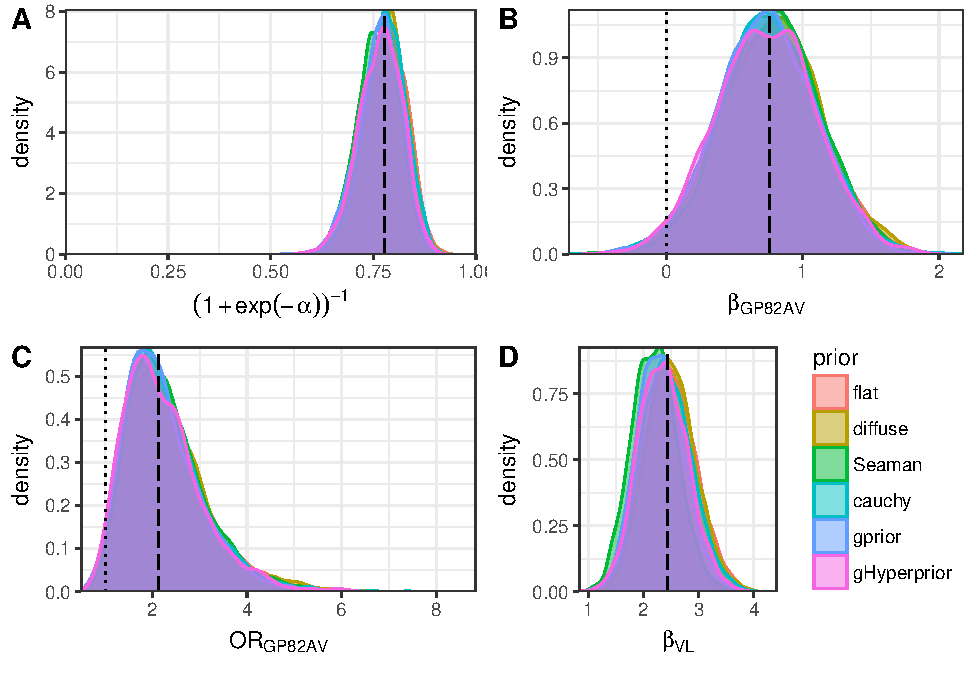
\includegraphics[scale=0.8]{\dir/figs/simple_logistic_PSA.pdf}
\caption[Prior sensitivity analysis for a simple logistic regression.]{\textbf{Prior sensitivity analysis for a simple logistic regression.}
In total I considered seven ``default'' priors routinely employed in the literature (see Section~\ref{sec:priors} for details).
Panel A shows the posterior distribution for the baseline CFR (a transformation of the intercept $\alpha$), while panel B shows the posterior distribution for the quantity of greater interest, the effect (coefficient) of GP82AV.
I show the resulting distribution on the odds ratio in panel C and the distribution of the coefficient for viral\_load in panel D.
The vertical dashed line shows the ordinary least squares parameter estimates and the dotted line indicates the null values $\beta_{\text{GP82AV}} = 0$ and $\text{OR} = 1$ for ease of comparison.
}
\label{fig:simpleLR}
\end{figure}

\subsection{Experiment 2: conservative and enthusiastic priors on the effect of GP82AV}
\label{sec:results-informative}

One might then be inclined to ask what the effect of incorporating external information and/or expert beliefs into the priors would be.
Since external information on the effects of a particular mutation in the virus and disease fatality and expert opinions on the subject are not available, I consider a simplified exercise where I construct conservative, neutral and optimistic priors for $\beta_{GP82AV}$.
While Figure~\ref{fig:informativePriors} shows these priors, Figure~\ref{fig:infomativePosteriors} presents the resulting posterior distributions for the parameters of a simple logistic regression.

\begin{figure}[!ht]
  \centering
  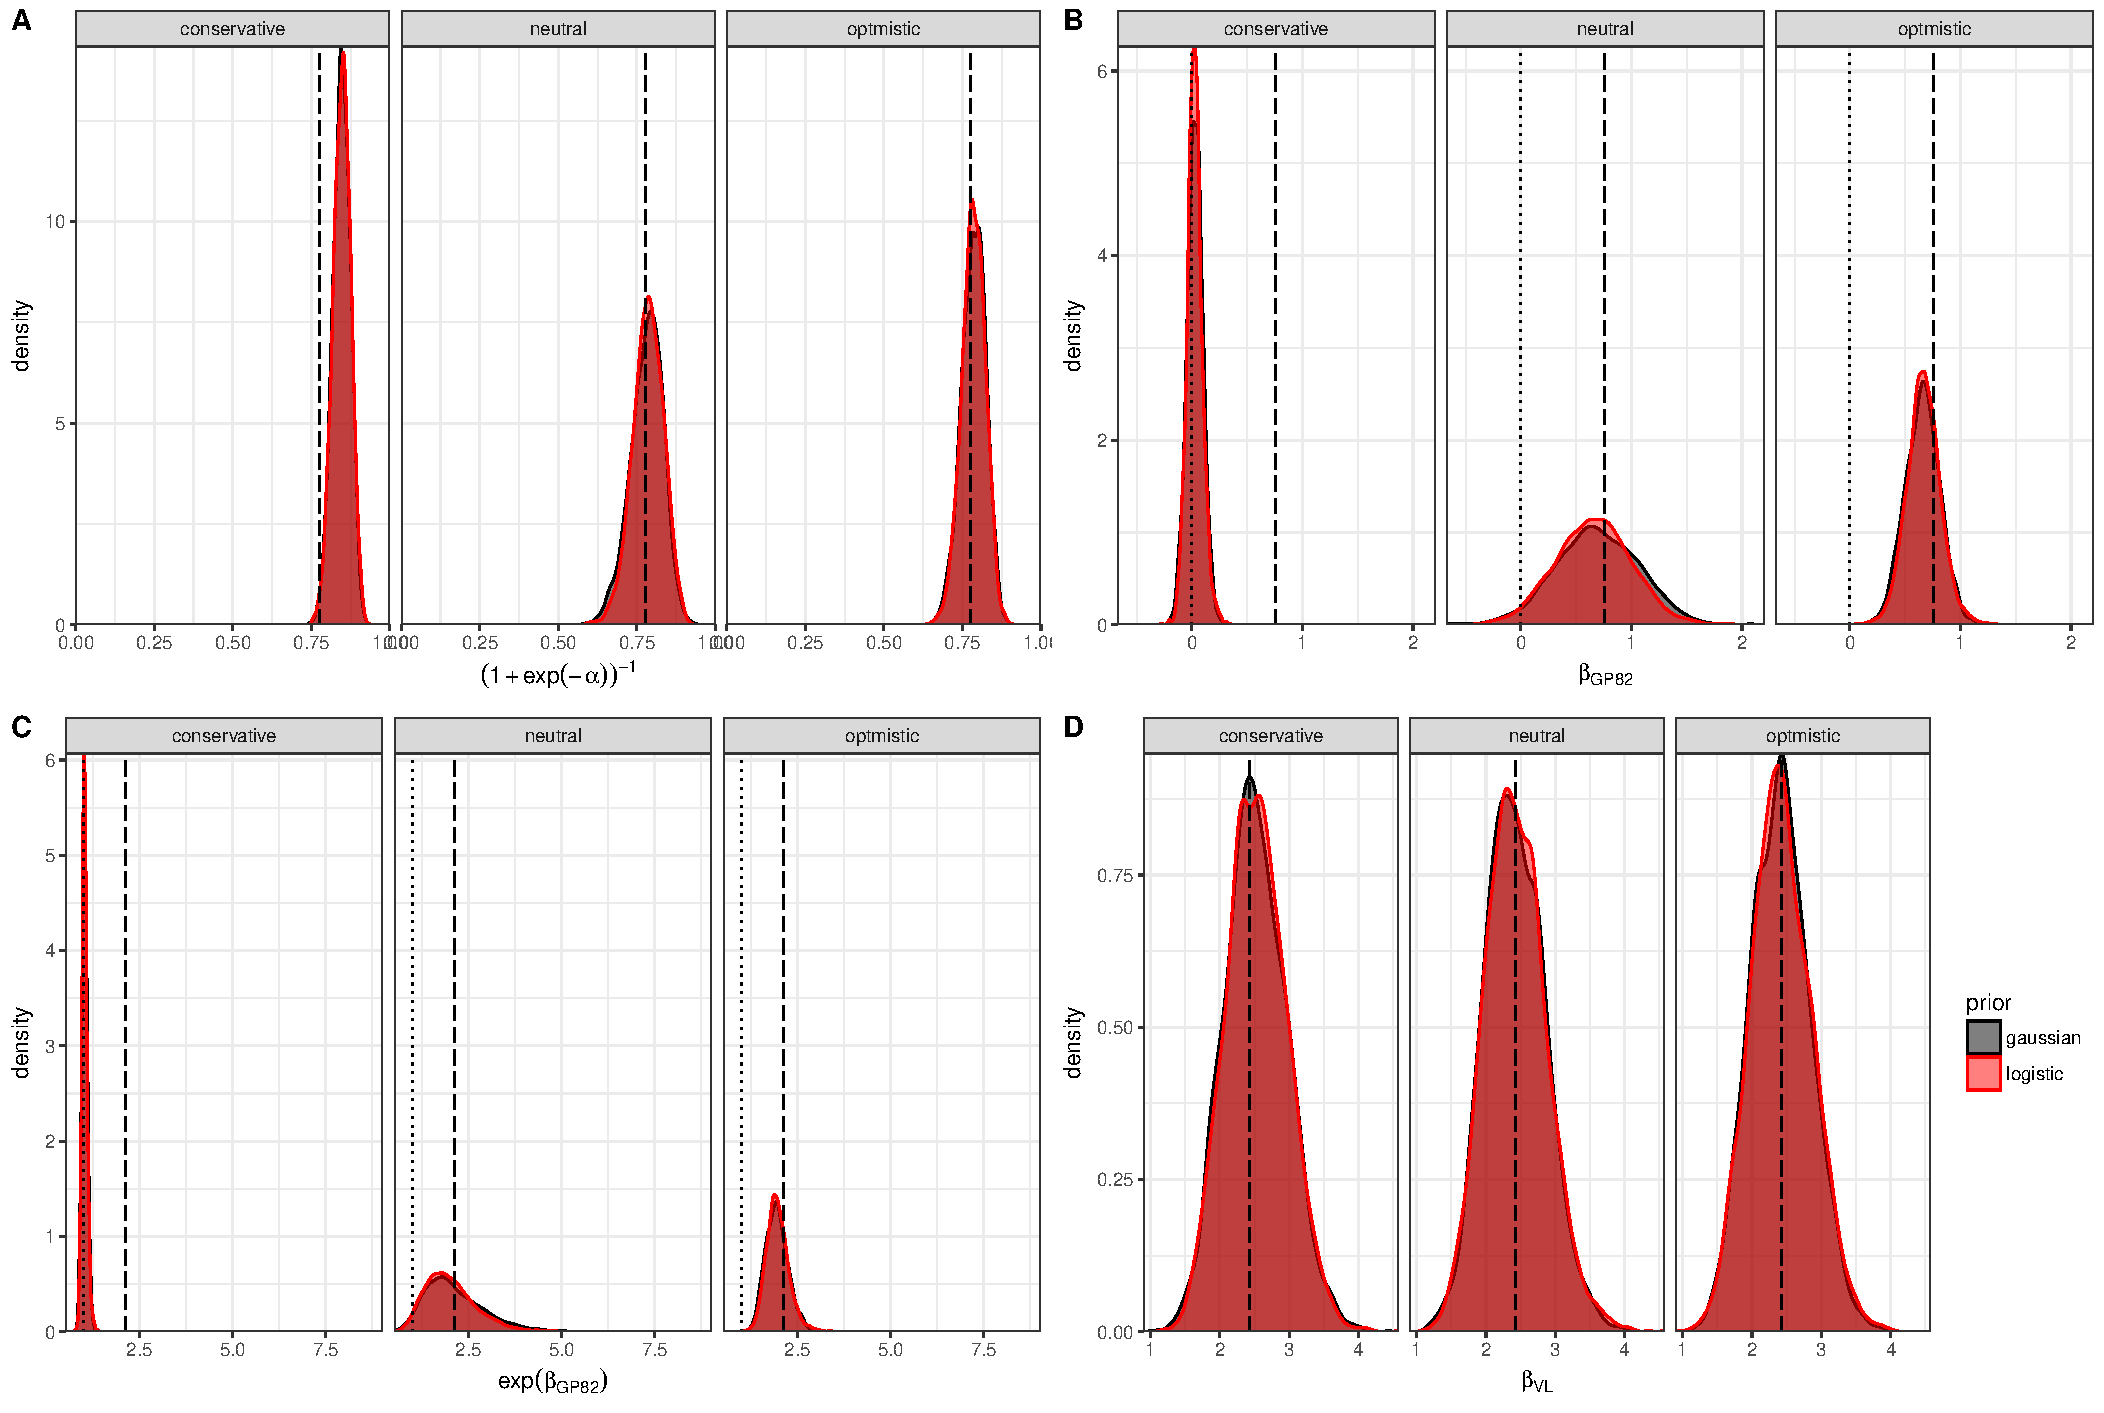
\includegraphics[scale=0.45]{\dir/figs/simple_logistic_informative_PSA.pdf}
\caption[Posterior distributions based on informative priors.]{\textbf{Posterior distributions based on informative priors.}
I show posterior distributions for the parameters of a simple logistic regression under the two families of distributions used to elicit conservative, neutral and optimistic priors for the effect of GP82AV.
The posterior for the baseline CFR is shown in panel A, while the coefficient and odds ratios for GP82AV are shown in panel B and C respectively.
Panel D shows the posterior distributions for the effect of the viral\_load predictor.
Dashed vertical lines show the OLS parameter estimates and dotted lines show the null values $\beta_{\text{GP82AV}} = 0$ and $\text{OR} = 1$ for ease of comparison.
}
\label{fig:infomativePosteriors}
\end{figure}

Posteriors obtained with different prior families (log-normal and log-logistic) are virtually indistinguishable, indicating that the importance of tail behaviour is negligible in this setting.
These sensitivity checks are important in order to gauge how informative the data are regarding the parameter of interest. 
In other words, the ability of the data to override (or not) different priors with different tail behaviours is a good indication of the amount of information contained in the data.

The first thing to notice is that the data are unable to change the prior beliefs under the conservative prior: posterior credibility intervals for the RR are virtually identical to the prior credibility interval $(0.95, 1.05)$.
As expected, the neutral priors behave similarly to the default priors studied in Section~\ref{sec:results-simple}. 
One key difference, however, is that posterior credibility intervals did include the ``null'' case of no effect; estimates for the odds ratio were $2.15$ $(0.97, 4.10)$ and $2.05$ $(0.95, 3.78)$ for the log-normal prior the log-logistic models, respectively.
Similarly, estimates for the risk ratio -- assuming $p_0 = 0.65$ as before -- were $1.20$ $(0.99, 1.36)$ and $1.19$ $(0.98, 1.35)$.
I hypothesise that these results are a consequence of the neutral prior explicitly accommodating the constraints imposed by the CFR, $p_0$, while the default priors previously considered allow risk ratios much bigger than $1.54$.

Somewhat counter-intuitively, in order to construct an optimistic prior -- under the two distribution families considered here -- one needs to construct priors that have more conservative upper bound.
The trade-off is to then have a prior that encodes a positive effect with greater certainty.
This is apparent from Figure~\ref{fig:informativePriors} and is reflected in the posterior RR estimates of $1.20$ $(1.11, 1.27)$ for the log-normal prior and $1.21$ $(1.12, 1.28)$ for the log-logistic.

\subsection*{Experiment 3: mutilevel modelling}
\label{sec:results-multilevel}

When considering the effect of the mutation on fatality rates, the cautious analyst would like to consider alternative explanations connected with the host population rather than the virus.
In other words, there might be confounding factors such as differential access to health care across locations, which could be driving the observed association between \verb|GP82AV| and risk of death.
I attempt to account for these factors by  formulating a model that explicitly accounts for variation in case fatality rates across locations through the model outlined in Equations~\ref{eq:varyingintA}~to~\ref{eq:varyingintB}.
The analyses in this section pertain to the data from Guinea only, since I could only reliably collect information on population-level predictors for that country.

The results in Figure~\ref{fig:multilevel} panel C show that there is substantial heterogeneity in case-fatality rates across locations, as evidenced by the bi-modal distribution of CFR for the model with no pooling (red density plot).
In panel B we see that assigning each location its own baseline case-fatality rate not only results in larger estimates for $\beta_{\text{GP82AV}}$ but also larger uncertainty, represented by the broader posterior.
This is to be expected since there is limited data per location and thus a model with no shrinkage is expected to produce noisier estimates. 
In addition, it is also likely that the sample data I analyse here is biased towards higher CFR, since these are cases that made it to the health care stage and therefore the sample likely excludes mild cases.
When partial pooling is employed, both with and without location-level predictors, we naturally see shrinking towards the overall mean (panel C).
The estimated CFR of $0.73$ $(0.55, 0.88)$ is still higher than the overall CFR for EVD computed by~\cite{Nyakarahuka2016} at $0.65$ $(0.54, 0.77)$.
According the World Health Organisation~\citep{WHO_2016b}, the CFR for the West African EVD outbreak was $0.76$ $(0.74, 0.77)$ for Guinea, $0.45$ $(0.44, 0.46)$ for Sierra Leone and $0.45$ $(0.44, 0.46)$ also for Liberia.
Since the sample analysed here (including previous sections) is dominated by Guinean samples, one would also expect to see a higher CFR.

\begin{figure}[!ht]
  \centering
  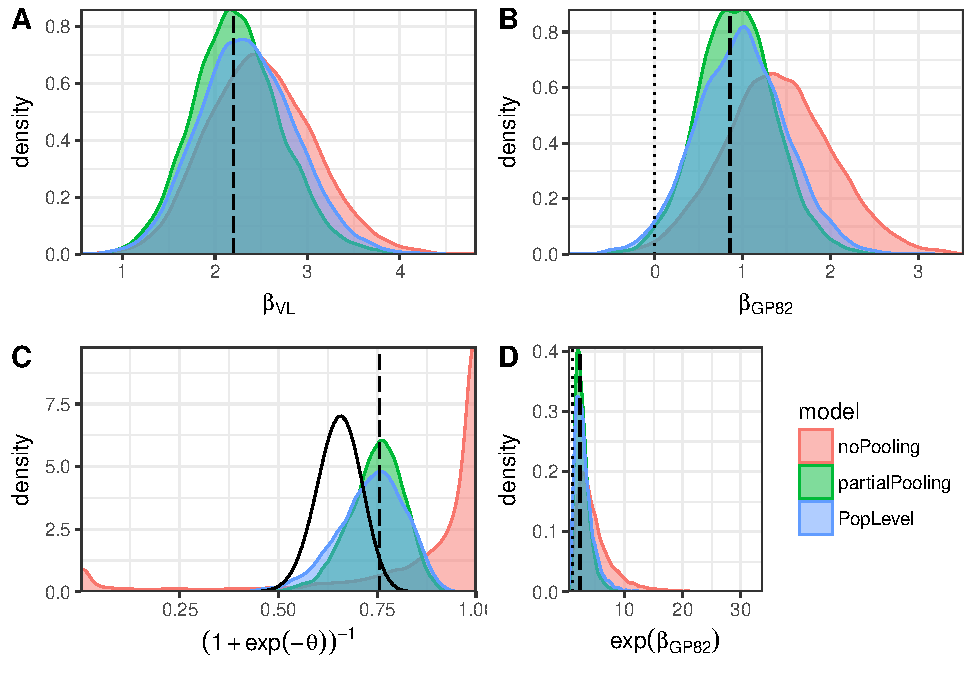
\includegraphics[scale=0.9]{\dir/figs/multilevel_logistic_MSA.pdf}
\caption[Posterior distributions for multilevel logistic models.]{\textbf{Posterior distributions for multilevel logistic models.}
I compare estimates under three models: no pooling (red), partial pooling without location-level predictors (green) and partial pooling including predictors (blue).
Panels A and B show the posterior distributions for the coefficients of viral\_load and GP82AV, respectively.
In panel C I show the posterior for the case-fatality rates through the appropriate transform of $\theta$.
For the no pooling model, I let $\theta = \frac{1}{J}\sum_{j=1}^J \alpha_j$.
Solid curve depicts the Beta prior I constructed in Section~\ref{sec:priors}.
Dashed vertical lines show the OLS parameter estimates and dotted lines show the null values $\beta_{\text{GP82AV}} = 0$ and $\text{OR} = 1$ for ease of comparison.
}
\label{fig:multilevel}
\end{figure}

It must be said that while I was able to gain some insight from these analyses, the ultimate goal of including population-level information to help explain differences in probability of death was not achieved.
This is because the posterior credibility intervals for the population-level coefficients $\boldsymbol\gamma$ included zero for all ten predictors considered, which indicates lack of significant association with the baseline case-fatality rate per location.
This finding could very well be the result of a limited sample size compared to the number of groups ($N = 202$, $J = 17$).

\subsection*{Experiment 4: accounting for shared ancestry}
\label{sec:results-phylo}

A key assumption of all the analyses presented so far is that of independence between observations.
Since EBOV is transmitted directly, this assumption is fundamentally violated.
Despite not being a perfect representation of the transmission history, the phylogeny $\tau$ reconstructed from the available sequences is a good proxy for the dependence structure in the data.
Accounting for this dependence is crucial in order to assess the effect of the mutation on fatality rates.
When I fitted a phylogenetic logistic regression model to the data using both \verb|GP82AV| and \verb|viral_load| as predictors, I obtained an estimate of $0.76$ with 95\% confidence interval $(-0.62, 2.13)$ for $\beta_{\text{GP82AV}}$, $2.13$ $(0.54, 8.45)$ for the odds ratio and $1.23$ $(0.77, 1.45)$ for the risk ratio.
It is clear from these estimates that once we account for the dependence between observations (sequences), the uncertainty about the estimates definitely precludes strong statements about the effect of \verb|GP82AV|.

The analysis of the association between \verb|viral_load| and phylogeny using the framework of~\cite{Vrancken2015} yielded $\lambda_B = 0.53 \: (0.29, 0.79)$.
These estimates point towards a moderate degree of phylogenetic signal,~\textit{i.e.} phylogeny-trait correlation.
In addition, the PLR analysis described previously also yielded estimates of the Ornstein-Uhlenbeck variance-restraining parameter $\alpha$ which are consistent with a significant association between the trait and phylogeny -- mean: $5.63$; 95\% parametric bootstrap interval: $(1.32, 76.33)$ -- despite a considerable amount of uncertainty.

\begin{figure}[!ht]
  \centering
  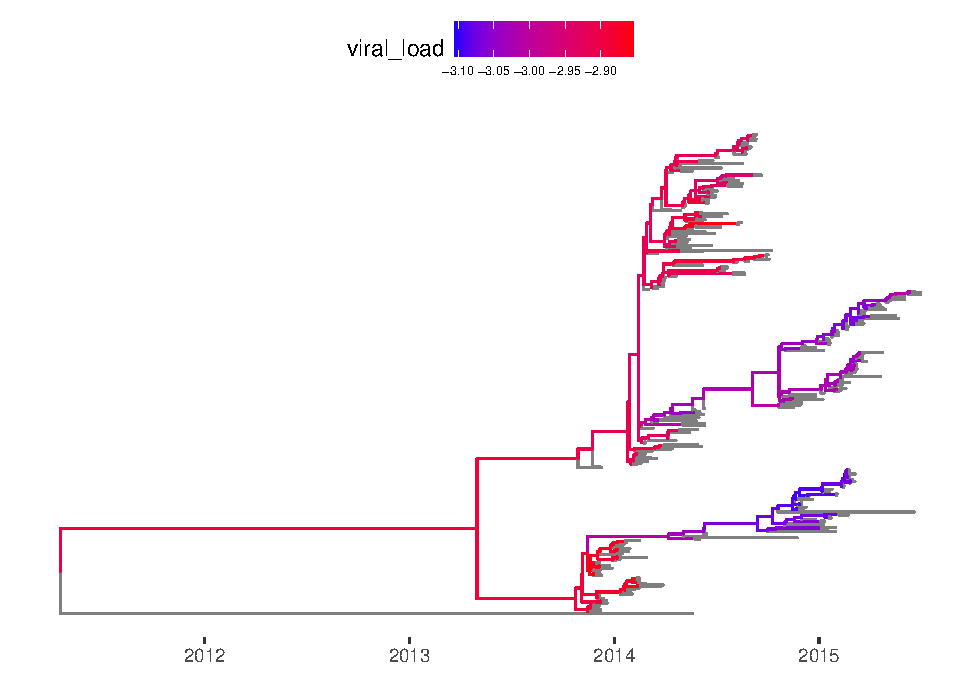
\includegraphics[scale=1.00]{\dir/figs/cta_viral_load_tree.pdf}
\caption[Time-calibrated phylogeny annotated with viral loads.]{\textbf{Time-calibrated phylogeny annotated with viral loads}.
I show inferred (posterior median) viral load values at internal branches using the Brownian motion continuous trait evolution model outlined in Section~\ref{sec:cta}.
Gray edges correspond to external nodes (tips).
}
\label{fig:CTAtree}
\end{figure}

An important observation is that from all the models considered in this study, higher viral loads are unequivocally associated with higher fatality rates.
Figure~\ref{fig:CTAtree} shows clear structure in viral load values across lineages, in agreement with the previous findings.
Taken together with the results from this section, this provides a possible explanation for the observed results: since viral load is moderately inheritable and the V mutation in GP emerged quite early -- in a deep branch --, the apparent association between \verb|GP82AV| and fatality might just be a result of latent dependence on the tree.
These findings reinforce the claim by~\cite{Russell2017} that the study and management of infectious diseases must be evolutionary, that is take into account evolutionary factors, the main of which is shared ancestry.

\subsection{Does GP82AV increase the risk of death from EVD?}

The short answer is: probably not.

The first issue to consider is that of \textbf{uncertainty}. 
In order to make claims about the effect of the \verb|GP82AV| mutation one needs first to quantify the uncertainty about the effect size.
As the analyses in Section~\ref{sec:MSerror} show, for a low true effect size (risk ratios $<1.10$), the standard error estimated with the current design/data could lead to gross overestimation of the effect. 
It must also be said that these analyses suggest that a sign error, that is an error that would lead to inferring \verb|GP82AV| to be a protective factor, is very unlikely.
If the mutation has any bearing on the outcome of EVD at all, it most likely increases the risk of dying.

With regard to the uncertainty about the baseline case-fatality rate ($p_0$), panel A in Figure~\ref{fig:ORRRuncertainty} shows the uncertainty about the maximum effect of the V mutation compared to the wild-type.
From this it is clear that it is very unlikely that being infected with a virus carrying the V mutation increases the probability of dying by more than $60$\%.
Panel B shows that the original estimate for $\beta_{\text{GP82AV}}$ lies in a region of large uncertainty w.r.t. risk ratios.
This means that, considering the variation (uncertainty) of the CFR, any estimate of the risk ratio corresponding  to the region of the observed log-odds ratio (taken at face value) could be between $1.15$ and $1.35$ with probability 95\%.

\begin{figure}[!ht]
  \centering
  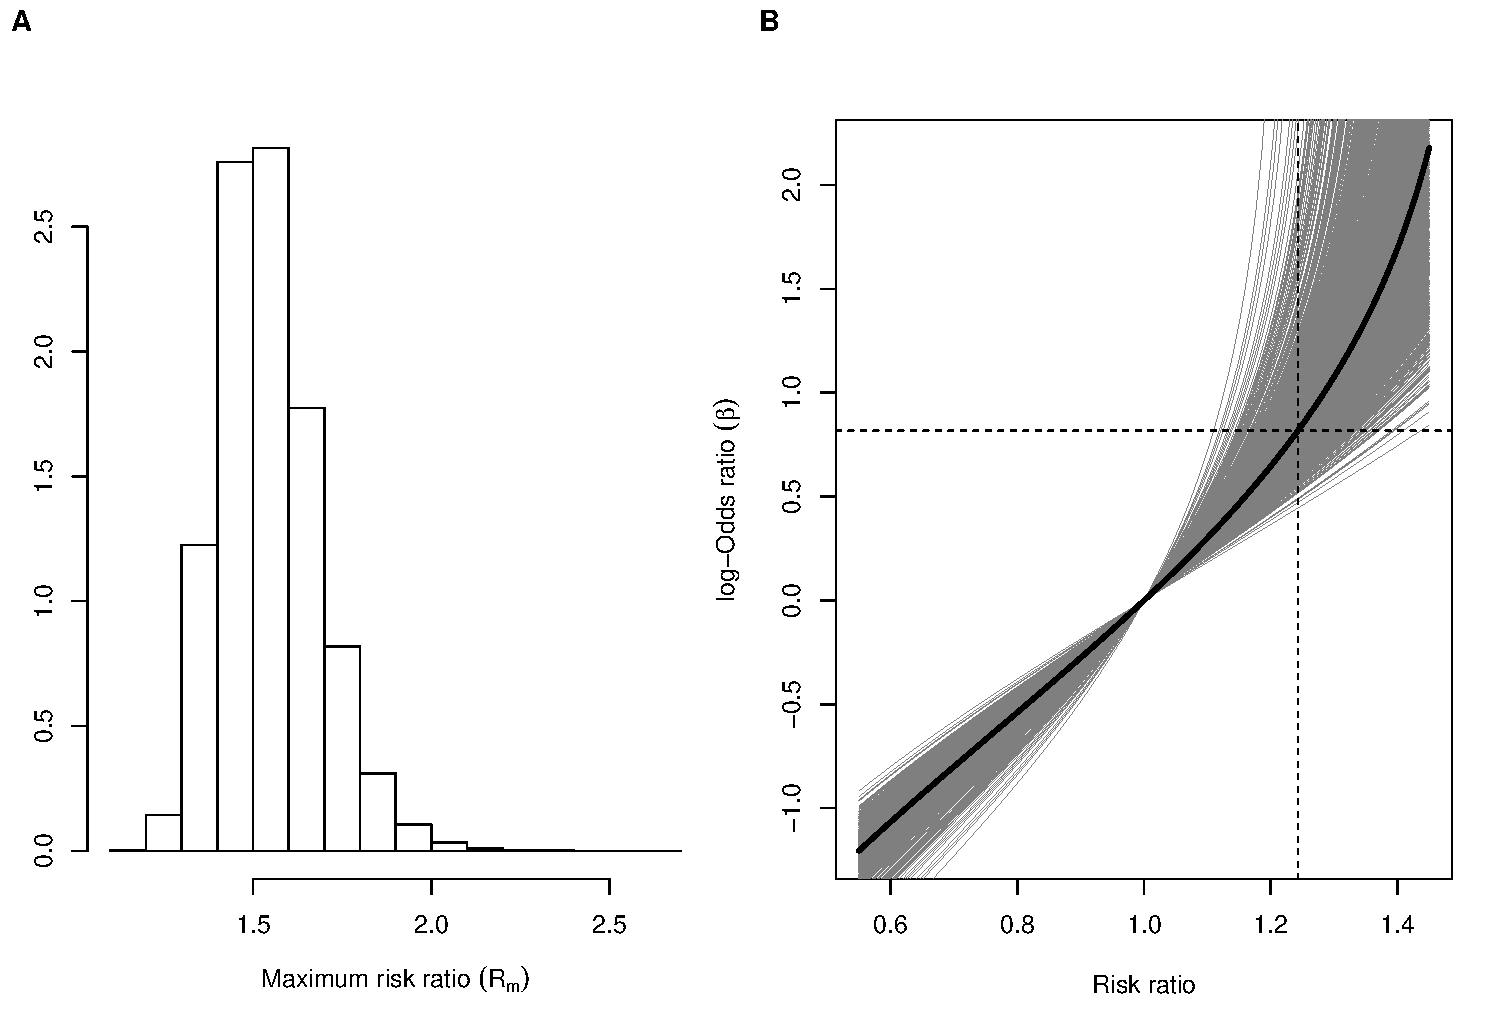
\includegraphics[scale=0.6]{\dir/figs/CFR_uncertainty_RR_OR.pdf}
\caption[Induced distributions on quantities of interest from the uncertainty about the case fatality ratio.]{\textbf{Induced distributions on quantities of interest from the uncertainty about the case fatality ratio (CFR), $p_0$}.
Using the distribution for $p_0$ constructed using the information in~\cite{Nyakarahuka2016} I explore the induced distributions on quantities of interest.  
In panel A I show the distribution of the maximum risk ratio ($R_m$).
panel B shows the relationship between (log) odds ratios,~\textit{i.e} the coefficient $\beta$, and risk ratios (eqs.~\ref{eq:ORRRa}~and~~\ref{eq:ORRRb}) through 1000 replicates from the distribution of $p_0$ (light grey lines).
Black solid line shows the relationship for $E[p_0] = 0.65$ and the dashed lines show the estimated coefficient for GP82AV ($\hat{\beta}_{GP82AV}$) and the corresponding risk ratio -- again with $E[p_0] = 0.65$.
}
\label{fig:ORRRuncertainty}
\end{figure}

A second point to consider is that of~\textbf{heterogeneity}.
From the results in Section~\ref{sec:results-multilevel} we see that there is considerable heterogeneity in fatality rates across locations, despite none of the included location-level predictors having a strong association with the baseline CFR.
When we account for heterogeneity across locations, we see that the effect of \verb|GP82AV| gets overshadowed by the uncertainty induced by the heterogeneity (Figure~\ref{fig:CFRpred}, left panel).
While there is still substantial separation between mean responses for both variants (GP82A and GP82V), the credibility intervals overlap considerably, preventing strong claims.

\begin{figure}[!ht]
  \centering
  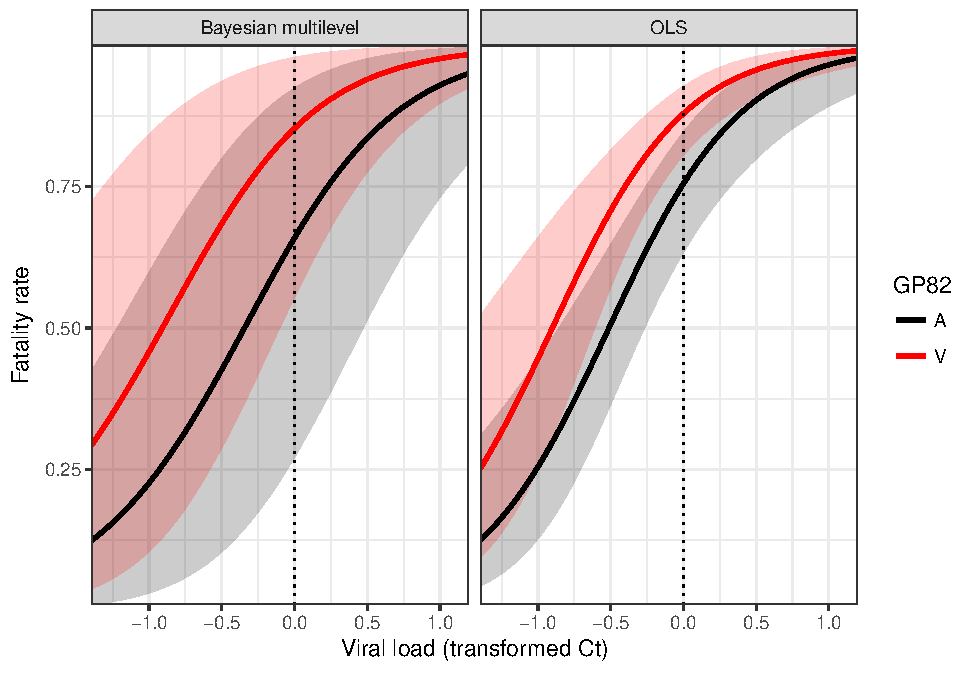
\includegraphics[scale=1.00]{\dir/figs/CFR_predictions.pdf}
\caption[Predicted case fatality ratio curves from OLS and Bayesian multi-level models.]{\textbf{Predicted case fatality ratio curves from OLS and Bayesian multi-level models}.
I show the predicted case-fatality rate curves for viral load (transformed \ct) for both genotypes (A: black, V: red). 
Vertical dotted line indicates the average viral load (recall the predictor is standardised) for ease of comparison.
}
\label{fig:CFRpred}
\end{figure}

The third point I propose considering is~\textbf{dependence}.
For instance, the methods in Section~\ref{sec:priors} rely heavily on the translation of risk ratios into odds ratios in order to elicit the prior distributions.
But as~\cite{Morozova2018} argue, risk ratios need careful interpretation when the outcome is contagious because transmissibility induces dependence between individuals.
The prior elicitation conducted here ignores this problem, although this could be relaxed in future research.
While exploring different sources of error, prior formulations and accounting for heterogeneity are all important, accommodating dependence between observations addresses a key assumption of my previous analyses.
Having access to complete genomes instead of, say, just genotyping information, allows us to estimate a phylogeny for the data points in study and hence obtain a proxy for the underlying dependence structure of the data.
The results from Section~\ref{sec:results-phylo} show that, after controlling for shared ancestry, the (bootstrap) confidence intervals for the effect of \verb|GP82AV| include the null hypothesis of no effect.


While I could combine all previous approaches into one single complicated model for further inquiry, it is my opinion that what we really need is more data and/or a better design.
Two final points worth considering are the roles of host heterogeneity and study design.
The data I analyse in this chapter unfortunately do not include important host (patient) information such as age, sex, pre-existing health conditions, etc.
It is entirely conceivable that heterogeneity in immune responses could be driving most of the variation in fatality rates.
Future efforts in matching patient data and available sequences may alleviate this problem by providing the missing information.

Even if more detailed patient information were available, however, the sample analysed here is one of convenience, collected as the epidemic progressed and patients were treated and tested at health care facilities, without a careful experimental design in mind.
This introduces biases that are hard to correct for (see for example the results in Section~\ref{sec:results-multilevel}).
A key insight is that if a mutation appears early on during an epidemic and then becomes fixed, it is difficult to disentangle its effects from other confounding factors at various levels, (exposure, geography, control measures, etc, see discussion in~\cite{Diehl2016}).
Conversely, if a mutation occurs repeatedly during an epidemic, we have much more scientific power to study its association with outcomes of interest such as fatality.
In other words, whether \verb|GP82AV| does indeed increase the chance of dying of EVD may not be answerable insofar as it may require direct experimentation in human subjects, which would be ethically unacceptable.
A recent study detailing experimentation in non-human subjects (mice and rhesus macaques) failed to show increased pathogenicity of \verb|GP82AV|~\citep{Marzi2018}.

\section{Conclusions}
\label{sec:conclusions}

In this chapter I lay out a principled analysis of the effects of a viral mutation on the fatality of the host.
I tackle the issue from multiple angles and, crucially, consider several sources of uncertainty.
When many sources of uncertainty about the effect of the \verb|GP82AV| mutation are considered, it is clear that strong claims are not warranted.
I also show that accounting for dependence between observations through the phylogeny leads to a substantial increase in uncertainty about the effect.
% Phylogenetic methods proved crucial to account for the dependence in the data and provide correct answers.
% The main lesson here is that all scientific statements, in order to be valid and useful, must be coupled with a proper account of the associated uncertainty and model assumptions.

% \bibliography{/home/max/Dropbox/PHD/THESIS/bibliography/lmcarvalho_PhD_Thesis}